\documentclass[12pt,a4paper]{article}
\usepackage[utf8]{inputenc}
\usepackage[spanish]{babel}
\usepackage{amsmath}
\usepackage{amsfonts}
\usepackage{amssymb}
\usepackage{graphicx}
\usepackage{geometry}
\usepackage{hyperref}
\usepackage{xcolor}
\usepackage{array}
\usepackage{booktabs}
\usepackage{fancyhdr}
\usepackage{titlesec}
\usepackage{float}

% Configuración de la página
\geometry{margin=2.5cm}

% Configuración de hyperref para índice hipervinculado
\hypersetup{
    colorlinks=true,
    linkcolor=blue,
    citecolor=red,
    urlcolor=blue,
    bookmarksnumbered=true,
    pdfstartview=FitH,
    pdftitle={Diferencia Fundamental entre Dirección y Sentido de un Vector},
    pdfauthor={[Autor]},
    pdfsubject={Análisis Vectorial}
}

% Configuración de encabezados y pies de página
\pagestyle{fancy}
\fancyhf{}
\fancyhead[L]{\leftmark}
\fancyhead[R]{\thepage}
\renewcommand{\headrulewidth}{0.4pt}
\renewcommand{\sectionmark}[1]{\markboth{#1}{}}

% Configuración de títulos
\titleformat{\section}{\Large\bfseries}{\thesection.}{1em}{}
\titleformat{\subsection}{\large\bfseries}{\thesubsection}{1em}{}
\titleformat{\subsubsection}{\normalsize\bfseries}{\thesubsubsection}{1em}{}

\title{\textbf{Diferencia Fundamental entre Dirección y Sentido de un Vector: Un Análisis Conceptual y Aplicado}}
\author{[Nombre del Autor]}
\date{\today}

\begin{document}
 
\maketitle

\newpage

% Índice hipervinculado
\tableofcontents
\newpage

\section{Introducción} \label{sec:introduccion}

En el lenguaje de la física y la ingeniería, los vectores son herramientas matemáticas de una importancia capital. Permiten describir y modelar magnitudes que, por su naturaleza, no pueden ser caracterizadas completamente por un único valor numérico, como la masa o la temperatura, conocidas como magnitudes escalares~\cite{grossman2012}. Magnitudes como la velocidad, la fuerza o el campo eléctrico exigen una especificación no solo de su intensidad, sino también de su orientación en el espacio~\cite{grossman2012}. Esta descripción completa se logra a través de los vectores.

Sin embargo, en el estudio de estas entidades matemáticas surge una confusión conceptual recurrente, especialmente entre los estudiantes que se inician en la materia: la distinción entre la dirección y el sentido de un vector. Con frecuencia, ambos términos se utilizan de manera intercambiable, lo que constituye un error fundamental~\cite{wikipedia_vector}. Esta no es una mera sutileza semántica, sino una distinción conceptual crítica cuyo dominio es un pilar para el análisis vectorial riguroso y la correcta aplicación de las leyes físicas~\cite{kolman2006}.

El objetivo de este informe es desambiguar de manera definitiva y exhaustiva la diferencia entre la dirección y el sentido de un vector. La tesis central que se defenderá es que la dirección define la orientación espacial de la línea de acción infinita sobre la que yace el vector, mientras que el sentido especifica una de las dos posibles orientaciones a lo largo de esa línea~\cite{wikipedia_vector}. Para demostrarlo, este documento se estructurará de la siguiente manera: se comenzará con las definiciones geométricas formales de cada concepto, se procederá a su representación y cuantificación analítica en sistemas de coordenadas, y se culminará con el análisis de casos de estudio prácticos en física e ingeniería, donde la distinción no solo es relevante, sino crucial para la correcta resolución de problemas y la seguridad de los diseños.
%figura 1
\begin{figure}[H]
    \centering
    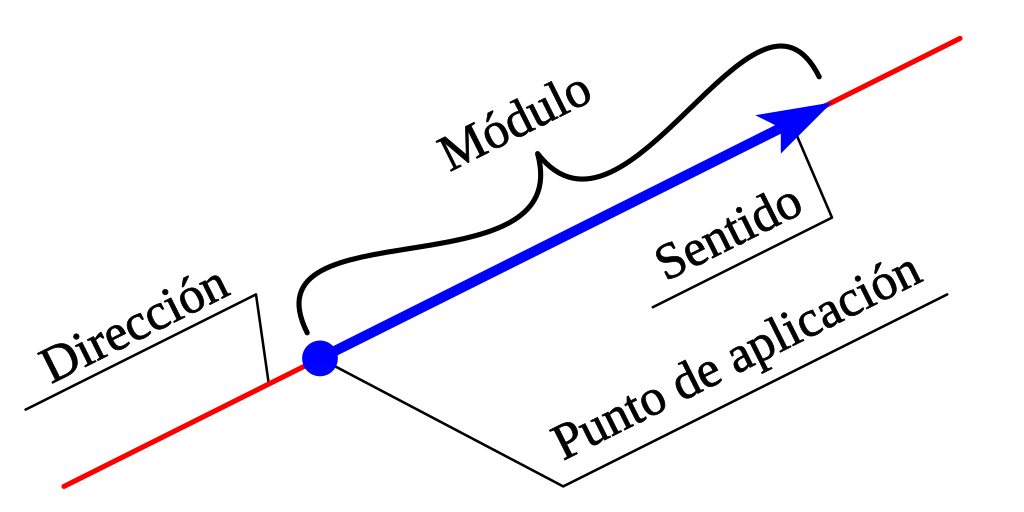
\includegraphics[width=0.6\textwidth]{1.png}
    \caption{Representación gráfica de un vector mostrando sus elementos fundamentales: módulo, dirección y sentido~\cite{wikipedia_vector}.}
    \label{fig:vector_intro}
\end{figure}

\section{Desarrollo} \label{sec:desarrollo}

\subsection{Fundamentos de las Magnitudes Vectoriales} \label{subsec:fundamentos}

Para comprender la diferencia entre dirección y sentido, es imperativo establecer primero una definición clara de lo que es un vector y cuáles son sus propiedades definitorias.

Geométricamente, un vector se concibe como un segmento de recta orientado dentro de un espacio euclidiano~\cite{wikipedia_vector}. Su representación gráfica más común es una flecha~\cite{wikipedia_vector}. Este segmento está unívocamente definido por un punto de origen (o punto de aplicación) y un punto final (o extremo)~\cite{kolman2006}. La esencia de un vector reside en tres características fundamentales que lo describen por completo, especialmente en el contexto de la lengua española:

\begin{enumerate}
\item \textbf{Módulo (o Magnitud):} Es la longitud del segmento de recta que representa al vector. Corresponde a la ``intensidad'' o ``tamaño'' de la magnitud física que se está modelando; por ejemplo, la magnitud de una fuerza en Newtons (N) o la rapidez de un objeto en metros por segundo (m/s). El módulo es siempre una cantidad escalar no negativa~\cite{grossman2012}. Se denota como $|\vec{v}|$ o simplemente $v$.

\item \textbf{Dirección:} Es la recta infinita que contiene al vector, también conocida como ``recta soporte'' o ``línea de acción''. Por extensión, la dirección también se refiere al conjunto de todas las rectas paralelas a esta línea de acción~\cite{kolman2006}.

\item \textbf{Sentido:} Es la orientación específica del vector sobre su línea de acción, la cual se indica gráficamente mediante la punta de la flecha. El sentido define ``hacia dónde'' apunta el vector a lo largo de su dirección~\cite{fernandez_coronado}.
\end{enumerate}

\subsection{Análisis Detallado de la Dirección Vectorial} \label{subsec:direccion}

La dirección es el atributo más amplio que define la orientación de un vector en el espacio. Formalmente, la dirección de un vector es la de su recta soporte. En consecuencia, dos o más vectores poseen la misma dirección si sus respectivas rectas soportes son paralelas, sin importar sus módulos o hacia dónde apunten sus flechas~\cite{superprof_vectores}.

Una analogía efectiva para visualizar este concepto es pensar en una autopista o una vía de tren~\cite{fastercapital}. La autopista en sí misma, extendiéndose indefinidamente en ambas orientaciones, representa una dirección. Todos los vehículos que se mueven sobre esa autopista, ya sea en un carril o en el otro, comparten la misma dirección de movimiento.

Gráficamente, un vector que se extiende de forma horizontal y otro que se extiende de forma vertical tienen direcciones distintas. Sin embargo, dos vectores horizontales, uno que apunta hacia la derecha y otro que apunta hacia la izquierda, comparten la misma dirección: la horizontal.

Analíticamente, en un sistema de coordenadas cartesiano bidimensional, la dirección se cuantifica de manera unívoca mediante el ángulo, comúnmente denotado por la letra griega theta ($\theta$), que la línea de acción del vector forma con un eje de referencia. Por convención, este eje suele ser el semieje positivo de las abscisas (eje X), y el ángulo se mide en sentido antihorario~\cite{grossman2012}. Todos los vectores paralelos entre sí, y por tanto con la misma dirección, formarán el mismo ángulo $\theta$ con dicho eje de referencia.

\subsection{Análisis Detallado del Sentido Vectorial} \label{subsec:sentido}

Una vez establecida una dirección, existen únicamente dos orientaciones posibles a lo largo de ella. El sentido es precisamente la elección de una de estas dos orientaciones~\cite{superprof_vectores}. Si la dirección es la autopista, el sentido corresponde al carril específico que se toma: el que va ``hacia el norte'' o el que va ``hacia el sur''~\cite{superprof_vectores}. Gráficamente, el sentido es representado de manera inequívoca por la punta de la flecha del vector~\cite{kolman2006}.

Este concepto es fundamental para definir los vectores opuestos. Dos vectores son opuestos si y solo si tienen el mismo módulo y la misma dirección, pero sentidos contrarios~\cite{serway2008}. Si un vector se denota como $\vec{v}$, su opuesto se representa como $-\vec{v}$. Gráficamente, serían dos flechas de igual longitud y paralelas, pero apuntando en orientaciones contrarias.

\subsection{Síntesis de la Distinción: Dirección vs. Sentido} \label{subsec:sintesis}

La relación entre dirección y sentido es jerárquica: la dirección es un concepto más general y fundamental, mientras que el sentido es una especificación subordinada a ella. No se puede definir un sentido sin haber establecido primero una dirección. La dirección establece la ``línea de juego'', y el sentido elige uno de los dos ``equipos'' o ``lados'' en esa línea.

Esta distinción se puede resumir de manera clara en la siguiente tabla comparativa:

\begin{table}[h]
\centering
\caption{Comparación Conceptual entre Dirección y Sentido}
\label{tab:comparacion}
\begin{tabular}{|>{\centering\arraybackslash}p{3cm}|>{\centering\arraybackslash}p{5.5cm}|>{\centering\arraybackslash}p{5.5cm}|}
\hline
\textbf{Característica} & \textbf{Dirección} & \textbf{Sentido} \\
\hline
Definición & La línea infinita que contiene al vector, o cualquier recta paralela a esta~\cite{wikipedia_vector} & Una de las dos posibles orientaciones sobre la línea de acción~\cite{fernandez_coronado} \\
\hline
Representación Gráfica & La inclinación de la recta soporte del vector~\cite{openstax_calculo} & La punta de la flecha del vector~\cite{fernandez_coronado} \\
\hline
Representación Analítica & El ángulo ($\theta$) que forma con un eje de referencia~\cite{ferrovial_vectores} & Los signos (+/-) de las componentes cartesianas del vector~\cite{openstax_fisica} \\
\hline
Analogía & Una calle de doble vía~\cite{superprof_vectores} & El carril específico por el que se circula en esa calle~\cite{superprof_vectores} \\
\hline
\end{tabular}
\end{table}

Es interesante notar que esta distinción conceptual tan marcada en la lengua española no siempre es tan explícita en otros idiomas. Por ejemplo, en inglés, la palabra \emph{direction} a menudo engloba tanto el concepto de dirección (orientación de la línea) como el de sentido (hacia dónde apunta la flecha)~\cite{wikipedia_vector}. En ese contexto, un vector se define por su \emph{magnitude} (módulo) y su \emph{direction}. Esta diferencia lingüística tiene una consecuencia pedagógica importante: el idioma español, al separar los términos, obliga a una mayor precisión conceptual desde el inicio del aprendizaje. Para un estudiante hispanohablante, comprender esta tricotomía (módulo, dirección y sentido) es un requisito impuesto por el propio lenguaje, lo que puede constituir una ventaja para evitar ambigüedades y construir una base conceptual más sólida y rigurosa desde el principio.

\subsection{Representación Analítica y Determinación} \label{subsec:representacion}

La transición del mundo geométrico al analítico se realiza mediante los sistemas de coordenadas. En un sistema cartesiano bidimensional, un vector $\vec{v}$ con origen en $(0,0)$ se representa por las coordenadas de su punto final, conocidas como sus componentes escalares $\langle v_x, v_y \rangle$~\cite{openstax_fisica}. Esta representación también se escribe en términos de los vectores unitarios $\hat{i}$ y $\hat{j}$ como $\vec{v} = v_x \hat{i} + v_y \hat{j}$~\cite{serway2008}.

La belleza de esta notación reside en cómo un simple par de números codifica eficientemente las tres propiedades del vector:

\subsubsection{Determinación del Módulo} \label{subsubsec:modulo}

El módulo $|\vec{v}|$ se calcula aplicando el teorema de Pitágoras a sus componentes, ya que estas forman los catetos de un triángulo rectángulo cuya hipotenusa es el vector mismo~\cite{grossman2012}:

\begin{equation}
|\vec{v}| = \sqrt{v_x^2 + v_y^2}
\end{equation}

Este cálculo depende de los valores al cuadrado de las componentes, por lo que es insensible a sus signos.

\subsubsection{Determinación de la Dirección} \label{subsubsec:dir_calc}

La dirección, representada por el ángulo $\theta$ con el eje X positivo, se obtiene de la relación trigonométrica entre las componentes:

\begin{equation}
\theta = \arctan\left(\frac{v_y}{v_x}\right)
\end{equation}

Es crucial ajustar el resultado de esta función, ya que la calculadora devuelve un ángulo en un rango limitado. El cuadrante correcto, y por tanto el ángulo final, se determina observando los signos de $v_x$ y $v_y$~\cite{openstax_fisica}.

\subsubsection{Determinación del Sentido} \label{subsubsec:sent_calc}

El sentido del vector queda inequívocamente determinado por los signos de sus componentes, que indican la orientación a lo largo de cada eje~\cite{openstax_fisica}:

\begin{itemize}
\item $v_x > 0$: Sentido hacia la derecha (eje X positivo)
\item $v_x < 0$: Sentido hacia la izquierda (eje X negativo)
\item $v_y > 0$: Sentido hacia arriba (eje Y positivo)  
\item $v_y < 0$: Sentido hacia abajo (eje Y negativo)
\end{itemize}

De este modo, las componentes cartesianas contienen una información dual. Sus valores absolutos determinan la magnitud del vector y la pendiente de su línea de acción (la dirección), mientras que sus signos algebraicos definen de manera precisa su sentido en el plano. Esta compactación de información es un claro ejemplo de la elegancia y eficiencia de la representación analítica de los vectores.

\subsection{Relevancia de la Distinción en Aplicaciones Prácticas} \label{subsec:aplicaciones}

La diferencia entre dirección y sentido no es un mero ejercicio académico; tiene consecuencias físicas y de ingeniería directas y, a menudo, críticas. Un error en la determinación del sentido puede invertir completamente el resultado de un cálculo, llevando a conclusiones erróneas o a fallos catastróficos en el diseño.

\subsubsection{Física de Campos: Fuerzas Eléctricas y Magnéticas} \label{subsubsec:campos}

En el estudio del electromagnetismo, la distinción es fundamental para predecir el movimiento de partículas cargadas.

\textbf{Campo Eléctrico ($\vec{E}$):} La fuerza eléctrica $\vec{F}_e$ que actúa sobre una partícula de carga $q$ inmersa en un campo eléctrico $\vec{E}$ viene dada por la expresión $\vec{F}_e = q\vec{E}$~\cite{serway2008}. La \emph{dirección} de la fuerza $\vec{F}_e$ es siempre la misma que la del campo $\vec{E}$ (son colineales). Sin embargo, el sentido de la fuerza depende críticamente del signo de la carga $q$. Si $q$ es positiva (como un protón), la fuerza tiene el mismo sentido que el campo. Si $q$ es negativa (como un electrón), la fuerza tiene el sentido opuesto al del campo~\cite{bariloche_web}.

%figura 2
\begin{figure}[H]
    \centering
    \includegraphics[width=0.6\textwidth]{2.png}
    \caption{Ilustración de la fuerza eléctrica sobre cargas positiva y negativa en un campo eléctrico uniforme~\cite{bariloche_web}.}
    \label{fig:fuerza_electrica}    
\end{figure}

\textbf{Campo Magnético ($\vec{B}$):} La fuerza magnética o fuerza de Lorentz, $\vec{F}_m$, sobre una carga $q$ que se mueve con velocidad $\vec{v}$ en un campo magnético $\vec{B}$ es $\vec{F}_m = q(\vec{v} \times \vec{B})$~\cite{bariloche_web}. La \emph{dirección} de esta fuerza es, por definición del producto vectorial, perpendicular al plano formado por los vectores $\vec{v}$ y $\vec{B}$. El sentido se determina mediante la regla de la mano derecha. No obstante, al igual que en el caso eléctrico, el sentido de la fuerza se invierte si la carga $q$ es negativa~\cite{bariloche_web}.

En aplicaciones como los selectores de velocidad, donde se busca que la fuerza eléctrica y la magnética se anulen, un error en el cálculo del sentido de cualquiera de las dos fuerzas llevaría a un diseño que, en lugar de seleccionar partículas con una velocidad específica, las desviaría a todas, haciendo el dispositivo completamente inoperante~\cite{bariloche_web}.

\subsubsection{Ingeniería Estructural: Análisis de Armaduras} \label{subsubsec:estructural}

En ingeniería civil, las armaduras o cerchas son estructuras compuestas por barras rectas unidas en sus extremos (nudos) para formar, por lo general, una red de triángulos. Se utilizan ampliamente en la construcción de puentes y techos~\cite{benguria_armaduras}. El método de los nudos es una técnica estándar para calcular las fuerzas internas que soporta cada barra~\cite{benguria_armaduras}.

En este análisis, la dirección de la fuerza en cada barra coincide con el eje longitudinal de la misma. El análisis de equilibrio en cada nudo (aplicando $\sum F_x = 0$ y $\sum F_y = 0$) permite calcular la magnitud de estas fuerzas. Sin embargo, el resultado más crítico de este cálculo es el signo de la fuerza, que determina su sentido.

\begin{itemize}
\item \textbf{Tensión (T):} Si la fuerza calculada es positiva (asumiendo inicialmente que la barra ``jala'' del nudo), significa que la barra está siendo estirada~\cite{benguria_armaduras}.

\item \textbf{Compresión (C):} Si la fuerza calculada es negativa, significa que la suposición inicial era incorrecta y la barra en realidad ``empuja'' al nudo, es decir, está siendo comprimida~\cite{benguria_armaduras}.
\end{itemize}

Esta distinción matemática entre dos sentidos opuestos tiene una consecuencia física fundamental. Una barra delgada diseñada para soportar tensión puede pandear y colapsar con una carga de compresión mucho menor. A la inversa, una unión diseñada para compresión podría fallar si se somete a tensión. Por lo tanto, un simple error de signo en el cálculo vectorial, un error en la determinación del sentido de la fuerza interna, puede traducirse directamente en un modelo de diseño incorrecto y, en el peor de los casos, en el colapso de una estructura real como un puente~\cite{scribd_aplicaciones}.

\subsubsection{Cinemática y Navegación: Composición de Velocidades} \label{subsubsec:cinematica}

El movimiento relativo es otro campo donde la distinción es crucial. Considérese el problema clásico de un bote que intenta cruzar un río con una corriente~\cite{serway2008}. La velocidad del bote respecto a la orilla ($\vec{v}_{\text{res}}$) es la suma vectorial de la velocidad que el bote tendría en aguas tranquilas ($\vec{v}_{\text{bote}}$) y la velocidad de la corriente del río ($\vec{v}_{\text{río}}$)~\cite{serway2008}:

\begin{equation}
\vec{v}_{\text{res}} = \vec{v}_{\text{bote}} + \vec{v}_{\text{río}}
\end{equation}

Para resolver este problema, es indispensable tratar cada velocidad como un vector con sus tres componentes bien definidas. Por ejemplo, supongamos que un bote puede moverse a 60 km/h y el río tiene una corriente de 15 km/h~\cite{serway2008}.

\begin{itemize}
\item \textbf{Caso A: Misma dirección y sentido (viaje río abajo).} Los vectores son colineales y apuntan en la misma orientación. La magnitud de la velocidad resultante es la suma de las magnitudes: $v_{\text{res}} = 60 + 15 = 75$ km/h.

\item \textbf{Caso B: Misma dirección, sentido opuesto (viaje río arriba).} Los vectores son colineales pero apuntan en orientaciones opuestas. La magnitud resultante es la resta: $v_{\text{res}} = 60 - 15 = 45$ km/h.

\item \textbf{Caso C: Direcciones perpendiculares (cruce del río).} Si el bote apunta perpendicularmente a la corriente, los vectores forman un triángulo rectángulo. La magnitud de la velocidad resultante se calcula con el teorema de Pitágoras: $v_{\text{res}} = \sqrt{60^2 + 15^2} \approx 61.8$ km/h. La dirección de su trayectoria real será un ángulo $\theta = \arctan(15/60) \approx 14.04°$ respecto a su rumbo original.
\end{itemize}

Este principio es la base de la navegación aérea y marítima~\cite{tripod_cinematica}. Los pilotos y capitanes utilizan constantemente el ``triángulo de velocidades'' para calcular su rumbo y velocidad verdaderos respecto a tierra, teniendo en cuenta el efecto del viento o las corrientes marinas~\cite{tripod_cinematica}. Un error en la determinación del \emph{sentido} del vector del viento (por ejemplo, considerarlo viento de cola cuando es viento en contra) llevaría a cálculos de tiempo de viaje, consumo de combustible y posición final drásticamente erróneos, con implicaciones directas para la seguridad de la operación.

\subsection{Extensiones y Contextos Avanzados} \label{subsec:extensiones}

Si bien la distinción euclidiana entre dirección y sentido es fundamental, es importante reconocer que constituye el primer escalón hacia conceptos más abstractos y potentes de orientación en marcos matemáticos y físicos superiores.

\textbf{Álgebra Geométrica (de Clifford):} En este formalismo matemático, que unifica el álgebra vectorial, los números complejos y los cuaterniones, los vectores pueden multiplicarse para generar objetos de mayor grado. El producto de dos vectores da lugar a un bivector, que representa un plano orientado. El concepto de ``sentido'' se generaliza al de ``orientación'' de este plano, que puede ser horaria o antihoraria. De manera similar, los trivectores representan volúmenes orientados (quiralidad).

\textbf{Relatividad General:} En la descripción de Einstein del espaciotiempo curvo, los vectores se definen localmente en ``espacios tangentes'' asociados a cada punto de la variedad espaciotemporal. Las partículas en caída libre siguen trayectorias llamadas geodésicas, que son las curvas ``más rectas'' posibles en dicha geometría. El vector tangente a una geodésica, análogo al vector velocidad clásico, es crucial para describir el movimiento, pero su significado está anclado a la estructura local del espaciotiempo.

El dominio de la distinción elemental entre dirección y sentido en el espacio euclidiano no es, por tanto, un fin en sí mismo, sino el requisito conceptual indispensable para acceder a estas descripciones más sofisticadas y precisas del universo físico y matemático.

\section{Conclusiones} \label{sec:conclusiones}

Este informe ha establecido una distinción clara, rigurosa y exhaustiva entre los conceptos de dirección y sentido de un vector. Se ha demostrado que no son sinónimos, sino propiedades jerárquicamente relacionadas y conceptualmente distintas~\cite{wikipedia_vector}. La \emph{dirección} es la cualidad que define la línea de acción de un vector en el espacio, respondiendo a la pregunta ``¿a lo largo de qué línea?''. Por su parte, el \emph{sentido} es la cualidad que especifica la orientación sobre esa línea, respondiendo a la pregunta ``¿hacia qué extremo de esa línea?''~\cite{wikipedia_vector}.

La importancia de esta distinción trasciende la mera corrección académica. Como se ha evidenciado a través de las aplicaciones analizadas, tiene implicaciones prácticas fundamentales:

\begin{itemize}
\item En física de campos, determina el sentido de la fuerza sobre partículas cargadas, un principio básico en el diseño de aceleradores y otros dispositivos electromagnéticos~\cite{bariloche_web}.

\item En ingeniería estructural, se traduce en la diferencia crítica entre tensión y compresión, donde un error de sentido en el cálculo puede comprometer la integridad y seguridad de una estructura~\cite{scribd_aplicaciones}.

\item En cinemática y navegación, es esencial para la composición de velocidades y el cálculo preciso de trayectorias, siendo un factor clave para la seguridad y eficiencia del transporte~\cite{serway2008}.
\end{itemize}

En definitiva, la comprensión precisa y la aplicación correcta de la diferencia entre dirección y sentido son un sello distintivo del rigor científico y técnico. Constituyen una habilidad conceptual básica que subyace a una vasta porción del análisis cuantitativo en las ciencias aplicadas. Su dominio no es opcional, sino un requisito esencial para cualquier estudiante o profesional que aspire a modelar y comprender el mundo físico de manera precisa y fiable.

\newpage

\begin{thebibliography}{20}

\bibitem{grossman2012}
S. I. Grossman y J. J. Flores Godoy, \emph{Álgebra Lineal}, 7ª ed. Ciudad de México, México: McGraw-Hill, 2012.

\bibitem{serway2008}
R. A. Serway y J. W. Jewett, \emph{Física para Ciencias e Ingeniería}, vol. 1, 7ª ed. Ciudad de México, México: Cengage Learning, 2008.

\bibitem{kolman2006}
B. Kolman y D. R. Hill, \emph{Álgebra Lineal}, 8ª ed. Naucalpan de Juárez, México: Pearson Educación, 2006.

\bibitem{wikipedia_vector}
Wikipedia, ``Vector'', 8 sep. 2025. [En línea]. Disponible en: \url{https://es.wikipedia.org/wiki/Vector}.

\bibitem{ferrovial_vectores}
Ferrovial, ``Vectores: qué son, características, tipos'', 2023. [En línea]. Disponible en: \url{https://www.ferrovial.com/es/stem/vectores/}.

\bibitem{superprof_vectores}
Superprof, ``Vectores'', [s.f.]. [En línea]. Disponible en: \url{https://www.superprof.es/apuntes/escolar/matematicas/analitica/vectores/vectores.html}.

\bibitem{fernandez_coronado}
J. L. Fernández y E. Coronado, ``Módulo, dirección y sentido'', Física con Sage, [s.f.]. [En línea]. Disponible en: \url{https://fisicaconsage.weebly.com/moacutedulo-direccioacuten-y-sentido.html}.

\bibitem{lima_platzi}
A. Lima, ``Respuesta a '¿Cuál es la diferencia entre dirección y sentido en un vector?'\,'', Platzi, hace 6 años. [En línea]. Disponible en: \url{https://platzi.com/discusiones/1278-algebra-lineal/58059-strongcual-es-la-diferencia-entre-direccion-y-sentido-en-un-vector-que-lo-determinastrong/}.

\bibitem{openstax_calculo}
OpenStax, ``Vectores en el plano'', Cálculo, Volumen 3, 2022. [En línea]. Disponible en: \url{https://openstax.org/books/c%C3%A1lculo-volumen-3/pages/2-1-vectores-en-el-plano}.

\bibitem{openstax_fisica}
W. Moebs, S. J. Ling, y J. Sanny, ``Álgebra de vectores'', Física universitaria volumen 1, 28 sep. 2021. [En línea]. Disponible en: \url{https://openstax.org/books/f%C3%ADsica-universitaria-volumen-1/pages/2-3-algebra-de-vectores}.

\bibitem{fastercapital}
FasterCapital, ``La importancia de la dirección en los cálculos de vectores'', [s.f.]. [En línea]. Disponible en: \url{https://fastercapital.com/es/tema/la-importancia-de-la-direcci%C3%B3n-en-los-c%C3%A1lculos-de-vectores.html/1}.

\bibitem{scribd_aplicaciones}
S. C. de Bariloche, ``Aplicación de los vectores en la ingeniería civil'', Scribd, [s.f.]. [En línea]. Disponible en: \url{https://es.scribd.com/document/723348396/LA-APLICACION-DE-LOS-VECTORES-EN-LA-INGENIERIA-CIVIL}.

\bibitem{bariloche_web}
S. B. Web, ``Movimiento de una carga en un campo eléctrico y magnético uniformes'', Física con ordenador, [s.f.]. [En línea]. Disponible en: \url{http://www.sc.ehu.es/sbweb/fisica3/magnetico/movimiento/movimiento.html}.

\bibitem{benguria_armaduras}
R. Benguria, ``Armaduras'', Pontificia Universidad Católica de Chile, [s.f.]. [En línea]. Disponible en: \url{http://www.fis.puc.cl/~rbenguri/ESTATICADINAMICA/Armaduras.pdf}.

\bibitem{tripod_cinematica}
D. Tripod, ``Cinemática Marítima'', 2020. [En línea]. Disponible en: \url{https://navegacion.tripod.com/webonmediacontents/7.01%20Cinematica%20Maritima%202020.pdf}.

\bibitem{udea_ieee}
Universidad de Antioquia, ``Guía rápida para el uso de las normas IEEE'', [s.f.]. [En línea]. Disponible en: \url{https://www.udea.edu.co/wps/wcm/connect/udea/9b7f1225-50ed-4266-b6c3-b5a9130bcc78/Gu%C3%ADa+r%C3%A1pida+para+el+uso+de+las+normas+IEEE.pdf?MOD=AJPERES&CVID=nRdL0sZ}.

\end{thebibliography}

\end{document}
